%%%%%%%%%%%%%%%%%%%%%%%%%%%%%%%%%%%%%%%%%%%%%%%%%%%%%
%		INTRODUCCION
%%%%%%%%%%%%%%%%%%%%%%%%%%%%%%%%%%%%%%%%%%%%%%%%%%%%%

\section[Introducci\'on]{Introducci\'on}
%\subsection{Introducci\'on}

\begin{frame}
\frametitle{Vidrios Metálicos}

\begin{itemize}
 \item Metal de estructura amorfa
 \item Basado en Cu, Ni, Fe, Au, Zr, Be, La, Pd, Ti
 \item Puede estar combinado en baja proporción con no metales como Bo, Si y P
 \item Combina propiedades de las cerámicas y de los metales
 \item Sus propiedades sobresalientes los hacen candidatos para aplicaciones modernas y de alta tecnología
\end{itemize}
\end{frame}

\definecolor{goodTitle}{HTML}{4D9A63}
\definecolor{goodDesc}{HTML}{A0DB8E}
\definecolor{alertTitle}{HTML}{FF2222}
\definecolor{alertDesc}{HTML}{FF9090}

\newcommand{\defaultBlocks}{
  \setbeamercolor{block title}{fg=white, bg=hsrmWarmGreyDark}
  \setbeamercolor{block body}{parent=palette secondary}
  \setbeamercolor{block title example}{fg=white, bg=hsrmSec1Dark}
  \setbeamercolor{block body example}{fg=white, bg=hsrmSec1}
  \setbeamercolor{block title alerted}{fg=white, bg=hsrmRedDark}
  \setbeamercolor{block body alerted}{fg=white, bg=hsrmRed}
}

\newcommand{\ventaja}[2]{
  \setbeamercolor{block title}{bg=goodTitle,fg=white}%
  \setbeamercolor{block body}{bg=goodDesc,fg=black}%
  \only<#1>{
    \begin{block}{Ventaja}%
    #2
    \end{block}%
   }
  \defaultBlocks%
}

\newcommand{\desventaja}[2]{
  \setbeamercolor{block title}{bg=alertTitle,fg=white}%
  \setbeamercolor{block body}{bg=alertDesc,fg=black}%
  \only<#1>{
    \begin{block}<#1>{Desventaja}%
    #2
    \end{block}%
   }
  \defaultBlocks%
}

\begin{frame}
\frametitle{Propiedades de los Vidrios Metálicos}
\begin{overprint}
 
\ventaja{1}{Ausencia de efectos adversos debidos a fronteras de granos}
\desventaja{1}{Alto costo y grandes limitaciones de fabricación}
    
\ventaja{2}{Alta dureza. Resistencia al desgaste y la abrasión. Gran resistencia mecánica y menor rigidez que las aleaciones cristalinas. Alta resiliencia}
\desventaja{2}{Gran pérdida de ductilidad ante la aparición de bandas de corte. El recocido lo vuelve frágil}

\ventaja{3}{Resistencia a la corrosión debido a la falta de bordes de grano}
\ventaja{3}{Algunos MG son biocompatibles}

\end{overprint}
\end{frame}

\begin{frame}
 \frametitle{Algunas aplicaciones de Vidrios Metálicos}
 
 \begin{figure}
 \centering
 \begin{tabularx}{\textwidth}{ccc}
 \only<1>{
 \subfloat[Filo estándar]{
    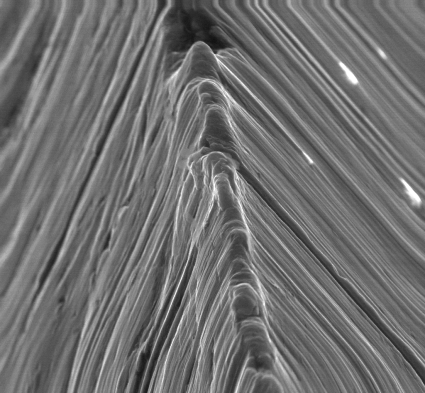
\includegraphics[width=3cm]{../Figures/Cap_1/blade.png}}
  &
  \subfloat[Filo de BMG]{
    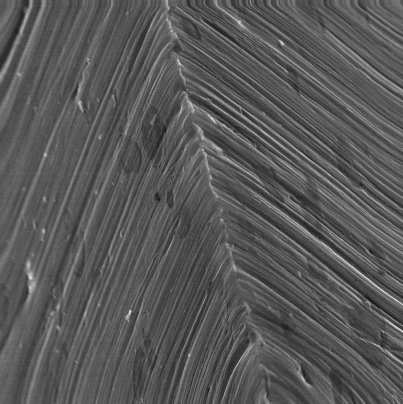
\includegraphics[width=3cm]{../Figures/Cap_1/BMG-blade.png}}
  &
  \subfloat[Joyería]{
    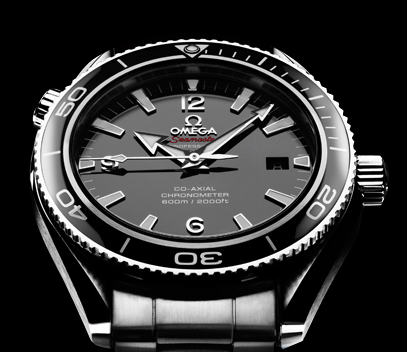
\includegraphics[width=3cm]{../Figures/Cap_1/seamaster.png}}
  }
  \only<2>{
  \subfloat[Deportes]{
    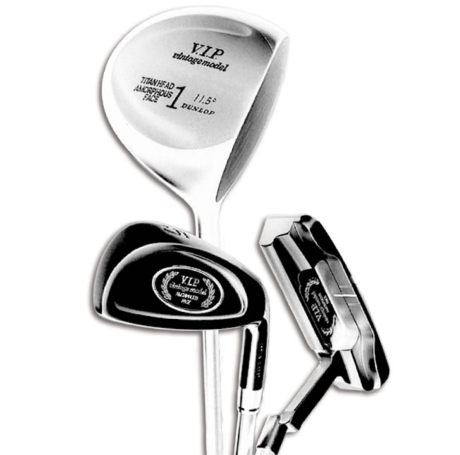
\includegraphics[width=3cm]{../Figures/Cap_1/golf.png}}
  &
  \subfloat[MEMS]{
    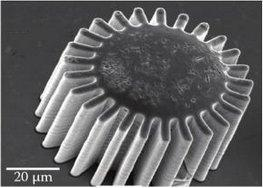
\includegraphics[width=3cm]{../Figures/Cap_1/MEMS_A.jpeg}}
  &
  \subfloat[MEMS]{
    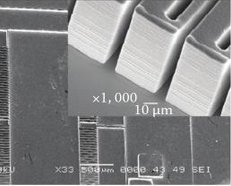
\includegraphics[width=3cm]{../Figures/Cap_1/MEMS_B.jpeg}}
    }
 \end{tabularx}
\end{figure}
\end{frame}

